%---------------------------------------------------------
%	PACKAGES AND THEMES
%---------------------------------------------------------

% https://ctan.math.utah.edu/ctan/tex-archive/macros/latex/contrib/beamer-contrib/themes/metropolis/doc/metropolistheme.pdf
\documentclass[aspectratio=169, 11pt]{beamer}

\usepackage{graphics}
\usepackage{pgfplots}
\pgfplotsset{width=15cm,compat=1.13,
            every axis/.append style={
                    label style={font=\large} 
                    }}
\usepgfplotslibrary{external}
\usepackage{pgfplotstable}
\usetikzlibrary{patterns}
\usepackage{tikz}
\usetikzlibrary{shapes,arrows,backgrounds,fit,positioning}
\tikzset{res/.style={ellipse,draw,minimum height=0.5cm,minimum width=0.8cm}}
\usepackage{multirow, hyperref}
\usepackage{wasysym}% Adds symbols

\usepackage{appendixnumberbeamer} % Restart number after appendix begins
\renewcommand{\appendixname}{\texorpdfstring{\translate{Appendix}}{Appendix}} % Because of bug

\usetheme[progressbar=foot, numbering=fraction]{metropolis}
%\setbeamertemplate{navigation symbols}{} % Removes the navigation symbols from the bottom of all slides

\definecolor{darkred}{rgb}{0.8,0,0}
\setbeamercolor{title separator}{fg=darkred}
\setbeamercolor{alerted text}{fg=orange}

\usepackage{graphicx} % Allows including images

% Define indicator ...
\DeclareSymbolFont{bbold}{U}{bbold}{m}{n}
\DeclareSymbolFontAlphabet{\mathbbold}{bbold}
\newcommand{\bi}{\mathbbold{1}}

% Deemphasize text
\newcommand{\light}{\textcolor{gray}}

\newcommand{\EE}{\mathbb{E}}
\newcommand{\PP}{\mathbb{P}}

%---------------------------------------------------------
%	TITLE PAGE
%---------------------------------------------------------

\title[Some title]{A title}

\author{Author names}
\date{A date}

% Road map
\AtBeginSection[]{%
\bgroup\setbeamertemplate{footline}{}% Hides slide counter
\addtocounter{framenumber}{-1}%        Doesn't add to slide counter
\begin{frame}{Outline}%
\tableofcontents[currentsection]%      Print ToC
\end{frame}\egroup%
}

% Doesn't increases page counter after every pause
%\resetcounteronoverlays{page}

\begin{document}

\maketitle

\section{First section}

\begin{frame}{A frame}
    
\end{frame}

\begin{frame}{Another frame}
    \only<3->{\hypertarget{example_to_return_to1}{}}
    This sentence contains an \alert{alerted} word!\pause
    
    And a second paragraph\only<2->{\footnote{A footnote}}\pause
    
    This is a link to the appendix. \hyperlink{app_example}{\texttt{link text}~ \beamerskipbutton{To appendix}}
\end{frame}

\section{Second section}

\begin{frame}{A frame with math}
    \begin{equation}
    \begin{aligned}
        y_{i,g,t} &= \beta \times \text{treatment}_g \times \text{post}_t \\
        &\qquad + \delta_i + \eta_t + X_{i,t} + \varepsilon_{i,g,t}.
    \end{aligned}
    \end{equation}
\end{frame}

\begin{frame}[plain, noframenumbering]
    \begin{center}
        \LARGE Thanks, the end, etc.
    \end{center}
\end{frame}

\AtBeginSection[]{}
\section{Appendix}

\appendix
% Appendix road map
\AtBeginSection[]{%
\begin{frame}{Appendix}
\tableofcontents[currentsection] %
\end{frame}%
}

\section{Extra: Appendix}

\begin{frame}{An appendix frame}
    With a Tikz graph!
    
    \begin{center}
    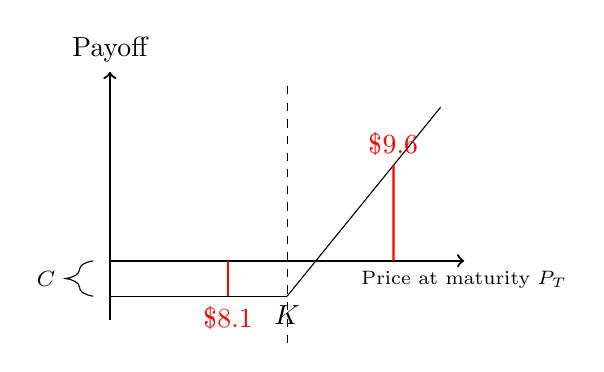
\begin{tikzpicture}[scale=1.5]
    % Draw axes
    \draw [<->,thick] (0,1.6) node (yaxis) [above] {Payoff}
        |- (3,0) node (xaxis) [below] {\scriptsize Price at maturity $P_T$};
    \draw [thick] (0,0) -- (0, -.5);
    
    \draw (0,-.3) -- (1.5,-.3) coordinate (K);
    \draw (K) node[below] {$K$} -- (2.8,1.3) coordinate (U);

    \draw [dashed] (1.5,-.7) -- (1.5, 1.5);
    
    \draw [decorate,decoration={brace,amplitude=10pt},xshift=-4pt,yshift=0pt]
    (0,-.3) -- (0,0) node [black,midway,xshift=-0.6cm] 
    {\footnotesize $C$};
    
    \coordinate (p_u)  at (2.4, 0);
    \coordinate (p_uu) at (2.4, 1);
    \coordinate (c) at (intersection of K--U and p_u--p_uu);
    
    \pause
    \draw [thick, red] (p_u) -- (c) node[above] {\$9.6};
    
    \pause
    \draw [thick, red] (1,0) -- (1,-0.3) node[below] {\$8.1};
    
    \end{tikzpicture}
    \end{center}
\end{frame}

\section{Appendix, part 2}

\begin{frame}[label=app_example]{Another appendix frame}
    With two different buttons that takes us back to the original page \quad \hyperlink{example_to_return_to1}{\beamerskipbutton{Go back}}\quad\hyperlink{example_to_return_to1}{\beamerbutton{Jump to}}
\end{frame}

\end{document}